\documentclass[conference, 10pt]{IEEEtran}
%\IEEEoverridecommandlockouts
% The preceding line is only needed to identify funding in the first footnote. If that is unneeded, please comment it out.
\usepackage{cite}
\usepackage{amsmath,amssymb,amsfonts}
\usepackage{algorithmic}
\usepackage{graphicx}
\usepackage{textcomp}
\usepackage{xcolor}
\usepackage[colorlinks = true,
            linkcolor = blue,
            urlcolor  = blue,
            citecolor = blue,
            anchorcolor = blue]{hyperref}
\usepackage[spanish,activeacute]{babel}

\def\BibTeX{{\rm B\kern-.05em{\sc i\kern-.025em b}\kern-.08em
    T\kern-.1667em\lower.7ex\hbox{E}\kern-.125emX}}
\begin{document}

\title{Problem Set 2: Predicting Poverty\\}

\author{\IEEEauthorblockN{Andrea Margarita Beleño}
\IEEEauthorblockA{200620739\\
E-mail:a.beleno@uniandes.edu.co}
\and
\IEEEauthorblockN{María Valeria Gaona}
\IEEEauthorblockA{202214418\\
E-mail:mv.gaona@uniandes.edu.co}
}

\maketitle

\begin{abstract}
En este Problem Set 2, se realizará la predicción de pobreza para los hogares de la Gran Encuesta integrada de Hogares 2018, utilizando
los métodos ROC, Falsos Positivos y Negativos, comparando dos modelos de categoría y de ingreso. El resultado, es que para el primer modelo, se utilizaron xx variables para la predicción, mientras que para el ingreso se utilizaron xx. El link al Github del presente taller, se encuentra en el siguiente enlace: \url{https://github.com/mvgaona/Problem-Set-N-mero-2}\\

\end{abstract}

\begin{IEEEkeywords}
component, formatting, style, styling, insert
\end{IEEEkeywords}

\section{Introducción}
Escribir la introducción del trabajo

\section{Datos}
La pobreza puede estar dada por diferentes variables. Sin embargo, es fundamental contar con las variables relevantes para que este modelo sea robusto, pero no se incurran en gastos que entorpezcan la investigación.\
La variable \textit{Npersug} (No. Personas en la unidad de gasto) evidencia aquellas personas que dentro del hogar están dentro de la unidad de gasto-UG. De acuerdo con el análisis, la moda de esta variable es 3, es decir, 3 personas por unidad de gasto es el valor más común entre unidades de gasto por familia. Además, se evidencia que el rango va de 1 a 28 personas por UG.\
La línea de pobreza (Lp) establece el límite de ingresos por debajo del cual un hogar es considerado pobre. El valor mínimo es COP 167.222;  el máximo COP 303.810,7; la media COP 271.605; la moda COP 281.549,3. Además, de acuerdo con DANE (2019) evidencia que la línea de pobreza monetaria nacional fue de \$257.433 pesos.\

La variable Dominio es una variable categórica que indica en donde vive el hogar. Existen 25 niveles, entre ellos Bogotá, Villavicencio, rural, entre otros. \


Se tomó la línea de pobreza definida por el DANE, que se encuentra en el documento publicado en el siguiente enlace: \url{https://www.dane.gov.co/files/investigaciones/condiciones_vida/pobreza/2018/bt_pobreza_monetaria_18.pdf}\\ 
\subsection{Por silas}

Frase por silas

\section{Modelo y Resultados}
Para comentar cualquier cosa \ref{AA}--\ref{SCM} below for more information on 
proofreading, spelling and grammar.

Keep your text and graphic files separate until after the text has been 
formatted and styled. Do not number text heads---{\LaTeX} will do that 
for you.

\subsection{Modelo de Clasificación}\label{AA}
Escribir los puntos relacionados en el problem set como:

\begin{itemize}
\item A detailed explanation of the final chosen model. The explanation must include how the model was trained, hyper-parameters selection, and other relevant information.
\item Include comparisons to at least 5 other models. You can compare them in terms of ROC, AUC, False Positives, or False Negatives.
\item Describe the variables that you used in the model and a measure of their
relative importance in the prediction. 
\item Describe any sub-sampling approach used to address class imbalances.
\end{itemize}


\subsection{Modelo del ingreso}
A continuación se describirá el proceso general para obtener el mejor modelo de regresión para realizar la predicción de pobreza utilizando este enfoque:




Se realizó el análisis de las variables en la base test para verificar que las variables contenidas en esta, estuvieran presentes en la de train para realizar la regresión con toda la información necesaria. Se llegó a la conclusión que para realizar esta regresión, se haría sobre la base de test de personas, obteniendo el ingreso por persona y realizar la sumatoria de los ingresos por cada persona del hogar y así tener el ingreso por hogar. Si bien este ingreso por hogar, se puede aproximar a la variable: \textit{Ingpcug}, mientras que la medición de pobreza se realiza con la variable \textit{Ingtotugarr}, para este ejemplo y considerando las siguientes estadísticas descriptivas para estas dos variables en la base de test, que se muestra en el Cuadro ~\ref{tab_1} :

\begin{table}[htbp]
\caption{Estadística descriptiva variables Ingpcug e Ingtotugarr}
\begin{center}
\begin{tabular}{|c|c|c|c|}
\hline
\textbf{Tabla}&\multicolumn{2}{|c|}{\textbf{Variables}} \\
\cline{2-3} 
\textbf{Estadístico} & \textbf{\textit{Ingpcug}}& \textbf{\textit{Ingtotugarr}} \\
\hline
Media& \$2.089.017&\$2.305.640\\
\hline
\end{tabular}
\label{tab_1}
\end{center}
\end{table}

Debido a que la diferencia del promedio entre un valor y otro es cercano al 10\% y considerando los posibles errores presentados en la predicción, obtenida a partir de la regresión, para calcular la pobreza a partir del ingreso se asumirá que: $Ingpcug\approx Ingtotugarr$.\\

Ahora bien, las variables escogidas para la regresión que se consideraron relevantes para el modelo, utilizando las teorías clásicas económicas, son las siguientes:

\begin{itemize}
\item Sexo
\item Edad y su componente cuadrática
\item Educación, representado en el nivel educativo más alto alcanzado por la persona
\item Ocupado: variable creada a partir de la variable \textit{Oficio}, para la cual, se tiene \textit{1} cuando existe el oficio y \textit{0} cuando no lo tiene. Se imputó el valor de cero en las bases de datos para los datos NA.
\item Dominio: Se consideró esta variable teniendo en cuenta que la línea de pobreza varía según la ciudad, por lo cual, se consideró relevante en el modelo.
\end{itemize}

Las anteriores variables, resultan en el siguiente modelo:\\
\begin{multline*}
Ingtot= \beta_{0}+\beta_{1}Edad+\beta_{2}Edad^{2}+\beta_{3}Sexo+\\
\beta_{4}Educacion+\beta_{5}Ocupado+\beta_{6}Dominio+u 
\end{multline*}

En primera instancia, se dividió la base de train de personas en un subtrain y subtest para mirar el ajuste del modelo y no tener overfitting, teniendo en cuenta que no se cuenta con la variable dependiente en el test para realizar una métrica más certera del modelo. Se realizó como primer modelo la regresión OLS, luego se realizaron varios modelos y la regularización con Ridge y Lasso para el modelo presentado en la ecuación anterior, así como pruebas de diferentes modelos con diferentes variables, que se presentan en las ecuaciones \eqref{eq:2}, \eqref{eq:3} y \eqref{eq:4}.


\begin{equation}
Ingtot= \beta_{0}+\beta_{1}Edad+\beta_{2}Edad^{2}+\beta_{3}Sexo+\\
\beta_{4}Educacion+u \label{eq:2}
\end{equation}

\begin{equation}
Ingtot= \beta_{0}+\beta_{1}Edad+\beta_{2}Edad^{2}+\beta_{3}Sexo+\\
\beta_{4}Educacion+\beta_{5}Ocupado+u \label{eq:3}
\end{equation}
\begin{equation}
Ingtot= \beta_{0}+\beta_{1}Edad+\beta_{2}Edad^{2}+\beta_{3}Sexo\label{eq:4}
\end{equation}

Para cada modelo con la base de train completa, mostrado en los modelos \eqref{eq:2}, \eqref{eq:3} y \eqref{eq:4}, se realizaron los modelos de Ridge y Lasso, se obtuvo el MSE de las predicciones sobre training y se realizó la gráfica que compara los modelos. Esta gráfica se encuentra en la Figura ~\ref{fig1}.  

\begin{figure}[htbp]
\centerline{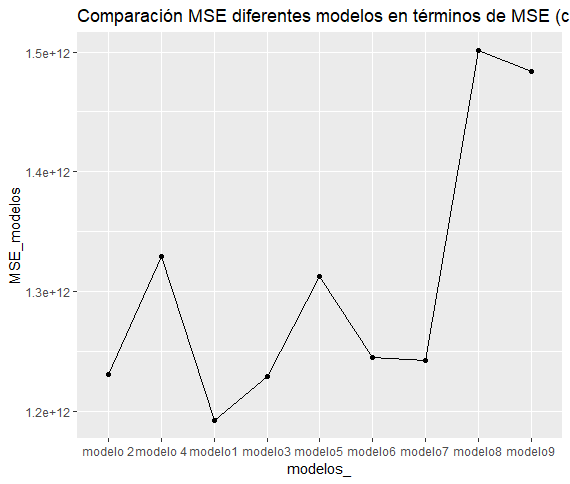
\includegraphics[width=0.4\textwidth]{../Vistas/MSE_base_training.png}}
\caption{Comparación MSE diferentes modelos base train personas}
\label{fig1}
\end{figure}

De dicha comparación, se obtiene que el modelo OLS (modelo 1) es el de menor MSE, por lo cual, es el que se escoge para realizar la regresión del Ingreso total por persona. No se reescaló el Ingreso (por ejemplo, con logaritmo), debido a que se busca obtener el valor y no una interpretación de este.\\
Para este modelo de regresión, el mejor modelo no fue obtenido por ningún hiperparámetro ni por ningún método de regularización, se escogió el de menor MSE, también porque en pruebas aleatorias, el parámetro Sensitivity fue mayor para este modelo OLS que para los obenidos de regularización.\\

Finalmente, la tabla de falsos positivos y negativos para el mejor modelo se presenta en la Figura ~\ref{fig2}, en donde para la predicción en el training se obtuvo un $Accuracy=$, y $Sensitivity=$.


\begin{itemize}
\item Include comparisons to at least 5 other models. Compare them in terms of
MSE.
\item Convert the predicted income to a binary indicator and show the performance in terms of the ROC, AUC, False Positives, or False Negatives.
\item Describe the variables that you used in the model and a measure of their relative importance in the prediction.
\end{itemize}


\section{Conclusiones y recomendaciones}

Se escriben las principales conclusiones y recomendaciones del ejercicio realizado anteriormente.

Lo que sigue es puro código que nos puede ayudar a ingresar fórmulas o datos chéveres en el paper.


The preferred spelling of the word ``acknowledgment'' in America is without 
an ``e'' after the ``g''. Avoid the stilted expression ``one of us (R. B. 
G.) thanks $\ldots$''. Instead, try ``R. B. G. thanks$\ldots$''. Put sponsor 
acknowledgments in the unnumbered footnote on the first page.

\subsection{Equations}
Number equations consecutively. To make your 
equations more compact, you may use the solidus (~/~), the exp function, or 
appropriate exponents. Italicize Roman symbols for quantities and variables, 
but not Greek symbols. Use a long dash rather than a hyphen for a minus 
sign. Punctuate equations with commas or periods when they are part of a 
sentence, as in:
\begin{equation}
a+b=\gamma\label{eq}
\end{equation}

Be sure that the 
symbols in your equation have been defined before or immediately following 
the equation. Use ``\eqref{eq}'', not ``Eq.~\eqref{eq}'' or ``equation \eqref{eq}'', except at 
the beginning of a sentence: ``Equation \eqref{eq} is . . .''



\subsection{Figures and Tables}
\paragraph{Positioning Figures and Tables} Place figures and tables at the top and 
bottom of columns. Avoid placing them in the middle of columns. Large 
figures and tables may span across both columns. Figure captions should be 
below the figures; table heads should appear above the tables. Insert 
figures and tables after they are cited in the text. Use the abbreviation 
``Fig.~\ref{fig}'', even at the beginning of a sentence.

\begin{table}[htbp]
\caption{Table Type Styles}
\begin{center}
\begin{tabular}{|c|c|c|c|}
\hline
\textbf{Table}&\multicolumn{3}{|c|}{\textbf{Table Column Head}} \\
\cline{2-4} 
\textbf{Head} & \textbf{\textit{Table column subhead}}& \textbf{\textit{Subhead}}& \textbf{\textit{Subhead}} \\
\hline
copy& More table copy$^{\mathrm{a}}$& &  \\
\hline
\multicolumn{4}{l}{$^{\mathrm{a}}$Sample of a Table footnote.}
\end{tabular}
\label{tab1}
\end{center}
\end{table}

\begin{figure}[htbp]
\centerline{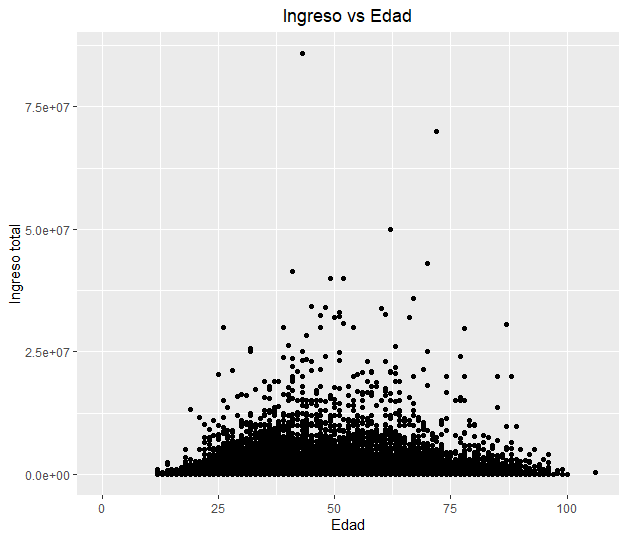
\includegraphics[width=0.4\textwidth]{../Vistas/Rplot01.png}}
\caption{Example of a figure caption.}
\label{fig}
\end{figure}

\begin{figure}[htbp]
\centerline{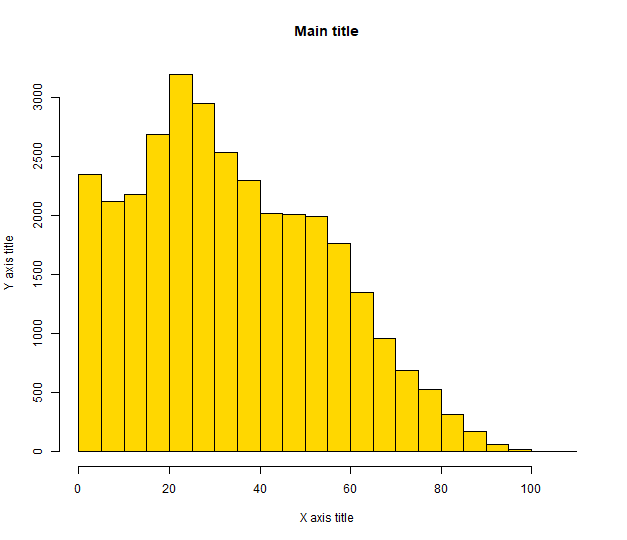
\includegraphics[width=0.4\textwidth]{../Vistas/Graficca_3.png}}
\caption{Example of a figure caption.}
\label{fig2}
\end{figure}

Figure Labels: Use 8 point Times New Roman for Figure labels. Use words 
rather than symbols or abbreviations when writing Figure axis labels to 
avoid confusing the reader. As an example, write the quantity 
``Magnetization'', or ``Magnetization, M'', not just ``M''. If including 
units in the label, present them within parentheses. Do not label axes only 
with units. In the example, write ``Magnetization (A/m)'' or ``Magnetization 
\{A[m(1)]\}'', not just ``A/m''. Do not label axes with a ratio of 
quantities and units. For example, write ``Temperature (K)'', not 
``Temperature/K''.



\section*{References}

Please number citations consecutively within brackets \cite{b1}. The 
sentence punctuation follows the bracket \cite{b2}. Refer simply to the reference 
number, as in \cite{b3}---do not use ``Ref. \cite{b3}'' or ``reference \cite{b3}'' except at 
the beginning of a sentence: ``Reference \cite{b3} was the first $\ldots$''

Number footnotes separately in superscripts. Place the actual footnote at 
the bottom of the column in which it was cited. Do not put footnotes in the 
abstract or reference list. Use letters for table footnotes.

Unless there are six authors or more give all authors' names; do not use 
``et al.''. Papers that have not been published, even if they have been 
submitted for publication, should be cited as ``unpublished'' \cite{b4}. Papers 
that have been accepted for publication should be cited as ``in press'' \cite{b5}. 
Capitalize only the first word in a paper title, except for proper nouns and 
element symbols.

For papers published in translation journals, please give the English 
citation first, followed by the original foreign-language citation \cite{b6}.

\begin{thebibliography}{00}
\bibitem{b1} G. Eason, B. Noble, and I. N. Sneddon, ``On certain integrals of Lipschitz-Hankel type involving products of Bessel functions,'' Phil. Trans. Roy. Soc. London, vol. A247, pp. 529--551, April 1955.
\bibitem{b2} J. Clerk Maxwell, A Treatise on Electricity and Magnetism, 3rd ed., vol. 2. Oxford: Clarendon, 1892, pp.68--73.
\bibitem{b3} I. S. Jacobs and C. P. Bean, ``Fine particles, thin films and exchange anisotropy,'' in Magnetism, vol. III, G. T. Rado and H. Suhl, Eds. New York: Academic, 1963, pp. 271--350.
\bibitem{b4} K. Elissa, ``Title of paper if known,'' unpublished.
\bibitem{b5} R. Nicole, ``Title of paper with only first word capitalized,'' J. Name Stand. Abbrev., in press.
\bibitem{b6} Y. Yorozu, M. Hirano, K. Oka, and Y. Tagawa, ``Electron spectroscopy studies on magneto-optical media and plastic substrate interface,'' IEEE Transl. J. Magn. Japan, vol. 2, pp. 740--741, August 1987 [Digests 9th Annual Conf. Magnetics Japan, p. 301, 1982].
\bibitem{b7} M. Young, The Technical Writer's Handbook. Mill Valley, CA: University Science, 1989.
\end{thebibliography}
\vspace{12pt}
\color{red}
IEEE conference templates contain guidance text for composing and formatting conference papers. Please ensure that all template text is removed from your conference paper prior to submission to the conference. Failure to remove the template text from your paper may result in your paper not being published.

\end{document}
